\chapter{Preliminaries and Distance Trees on Proper Interval Graphs}
\label{chap:prelim}

This chapter establishes the formal graph-theoretic foundations, definitions, geometric representation theorems, and structural machinery required throughout this thesis. We rigorously formalize interval graphs and proper interval graphs, prove the fundamental property of strict endpoint monotonicity, review classical intersection properties (the Helly property and chordality), and introduce the central analytical framework of this work: the \emph{canonical distance tree} $T(G)$.

\section{Graph-Theoretic Notation and Conventions}
\label{sec:prelim_notation}

Throughout this thesis, all graphs considered are finite, simple (containing no loops or multiple edges), and undirected unless explicitly stated otherwise. 

Let $G = (V, E)$ be a graph with vertex set $V(G) = V$ and edge set $E(G) = E$. We denote the number of vertices by $n = |V|$ and the number of edges by $m = |E|$. An edge between two distinct vertices $u, v \in V$ is denoted by $uv \in E$ (or equivalently $(u, v) \in E$). Two vertices $u, v$ are said to be \emph{adjacent} (or \emph{neighbors}) if $uv \in E$.

For a vertex $v \in V$:
\begin{itemize}
    \item The \emph{open neighborhood} of $v$ is the set of all vertices adjacent to $v$:
    \begin{equation}
        N(v) = \{ u \in V \mid uv \in E \}.
    \end{equation}
    \item The \emph{closed neighborhood} of $v$ includes $v$ itself:
    \begin{equation}
        N[v] = N(v) \cup \{ v \}.
    \end{equation}
    \item The \emph{degree} of $v$ is the cardinality of its open neighborhood: $d(v) = |N(v)|$.
\end{itemize}

A \emph{path} of length $k$ from $u$ to $w$ is a sequence of distinct vertices $\langle v_0, v_1, \dots, v_k \rangle$ such that $v_0 = u$, $v_k = w$, and $v_i v_{i+1} \in E$ for each $0 \le i < k$. The graph-theoretic \emph{distance} between $u$ and $w$, denoted by $d_G(u, w)$, is the minimum length of a path connecting $u$ and $w$ in $G$. If no such path exists, $d_G(u, w) = \infty$. The graph $G$ is \emph{connected} if $d_G(u, w) < \infty$ for all $u, w \in V$. The \emph{diameter} of a connected graph $G$, denoted by $\operatorname{diam}(G)$, is $\max_{u, v \in V} d_G(u, v)$.

A subset of vertices $K \subseteq V$ is a \emph{clique} if every pair of distinct vertices in $K$ is adjacent ($uv \in E$ for all $u, v \in K$ with $u \ne v$). A clique $K$ is a \emph{maximal clique} if no strictly larger clique in $G$ contains $K$ (i.e., for any vertex $w \in V \setminus K$, $K \cup \{w\}$ is not a clique). A clique is a \emph{maximum clique} if it achieves the maximum cardinality among all cliques in $G$; its size is the \emph{clique number} $\omega(G)$.

A subset of vertices $S \subseteq V$ is an \emph{independent set} (or \emph{stable set}) if no two vertices in $S$ are adjacent ($uv \notin E$ for all $u, v \in S$). An independent set is a \emph{maximum independent set} (MIS) if it has maximum cardinality; its size is the \emph{independence number} $\alpha(G)$.

A subset $D \subseteq V$ is a \emph{dominating set} if every vertex $v \in V \setminus D$ has at least one neighbor in $D$. The \emph{domination number} $\gamma(G)$ is the minimum cardinality of a dominating set in $G$.

\section{Interval Graphs and Proper Interval Graphs}
\label{sec:prelim_interval_graphs}

\begin{definition}[Interval Representation]
Let $G = (V, E)$ be a graph. An \emph{interval representation} of $G$ is a family of closed intervals on the real line:
\begin{equation}
    \mathcal{I} = \{ I_v = [l_v, r_v] \subset \mathbb{R} \mid v \in V, \; l_v \le r_v \},
\end{equation}
such that two vertices are adjacent in $G$ if and only if their assigned intervals have a non-empty intersection:
\begin{equation}
    \forall u, v \in V, \; u \ne v: \quad uv \in E \iff I_u \cap I_v \ne \emptyset.
\end{equation}
A graph admitting an interval representation is an \emph{interval graph}.
\end{definition}

Two closed intervals $I_u = [l_u, r_u]$ and $I_v = [l_v, r_v]$ intersect if and only if:
\begin{equation}
    l_u \le r_v \quad \text{and} \quad l_v \le r_u.
\end{equation}
Conversely, $I_u$ lies entirely to the left of $I_v$ (denoted $I_u \prec I_v$) if and only if $r_u < l_v$, in which case $uv \notin E$.

\begin{definition}[Proper Interval Graph]
An interval graph $G$ is a \emph{proper interval graph} if it admits an interval representation $\mathcal{I}$ in which no interval properly contains another, i.e.,
\begin{equation}
    \forall u, v \in V, \; u \ne v: \quad I_u \not\subset I_v.
\end{equation}
That is, there do not exist distinct vertices $u, v$ such that $l_v \le l_u \le r_u \le r_v$ with at least one strict inequality.
\end{definition}

Without loss of generality, by applying an infinitesimal topological perturbation that preserves all intersection relationships, we can assume that all interval endpoints in $\mathcal{I}$ are distinct:
\begin{equation}
    l_u \ne l_v \quad \text{and} \quad r_u \ne r_v \quad \forall u \ne v.
\end{equation}

\subsection{Strict Endpoint Monotonicity}

The fundamental structural property that separates proper interval graphs from general interval graphs is the preservation of linear order between left and right endpoints.

\begin{theorem}[Strict Endpoint Monotonicity]
\label{thm:endpoint_monotonicity}
Let $G = (V, E)$ be a proper interval graph with interval representation $\mathcal{I} = \{[l_v, r_v] \mid v \in V\}$ possessing distinct endpoints. For any two vertices $u, v \in V$:
\begin{equation}
    l_u < l_v \iff r_u < r_v.
\end{equation}
\end{theorem}
\begin{proof}
$(\Longrightarrow)$ Suppose $l_u < l_v$. We must show that $r_u < r_v$. Assume for the sake of contradiction that $r_u > r_v$. Then we have:
\[
    l_u < l_v < r_v < r_u.
\]
This implies that $I_v = [l_v, r_v]$ is strictly contained within the interior of $I_u = [l_u, r_u]$, i.e., $I_v \subset I_u$. This directly violates the definition of a proper interval representation. Hence, by contradiction, we must have $r_u < r_v$.

$(\Longleftarrow)$ Conversely, suppose $r_u < r_v$. If $l_u > l_v$, then $l_v < l_u < r_u < r_v$, which implies $I_u \subset I_v$, again violating properness. Thus, $l_u < l_v$.
\end{proof}

\begin{figure}[htbp]
    \centering
    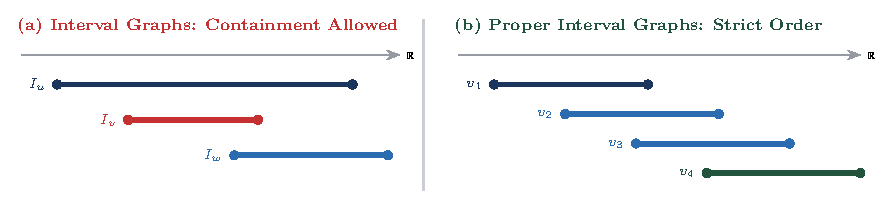
\includegraphics[width=0.92\linewidth]{figures/fig_intervals_distinction.pdf}
    \caption[Distinction between General and Proper Interval Graphs]{Distinction between (a) General interval graphs, where interval containment ($I_v \subset I_u$) is permitted and breaks endpoint monotonicity, and (b) Proper interval graphs, where strict monotonicity ($l_u < l_v \iff r_u < r_v$) enforces a unified left-to-right linear ordering.}
    \label{fig:intervals_distinction}
\end{figure}

\begin{definition}[Canonical Vertex Ordering]
Let $G$ be a proper interval graph. The \emph{canonical vertex ordering} is the sequence of vertices ordered by strictly increasing left endpoints:
\begin{equation}
    V = \{v_1, v_2, \dots, v_n\} \quad \text{such that} \quad l_{v_1} < l_{v_2} < \dots < l_{v_n}.
\end{equation}
By Theorem~\ref{thm:endpoint_monotonicity}, the right endpoints simultaneously satisfy:
\begin{equation}
    r_{v_1} < r_{v_2} < \dots < r_{v_n}.
\end{equation}
Throughout this thesis, when vertices are indexed as integers $1, 2, \dots, n$, the notation $u < v$ refers strictly to this canonical ordering ($l_u < l_v$).
\end{definition}

An immediate consequence of canonical ordering is that adjacency between vertices is \emph{contiguous}:
\begin{corollary}[Adjacency Contiguity]
\label{cor:adjacency_contiguity}
Let $G = (V, E)$ be a proper interval graph ordered canonically. If $u < w < v$ and $uv \in E$, then $uw \in E$ and $wv \in E$.
\end{corollary}
\begin{proof}
Since $uv \in E$ and $u < v$, we have $l_u < l_v \le r_u$. Because $u < w < v$, monotonicity gives $l_u < l_w < l_v$ and $r_u < r_w < r_v$. Thus:
\[
    l_w < l_v \le r_u < r_w \implies I_u \cap I_w \ne \emptyset \implies uw \in E,
\]
and
\[
    l_v \le r_u < r_w \implies l_w < l_v \le r_w \implies I_w \cap I_v \ne \emptyset \implies wv \in E.
\]
\end{proof}

\section{Classical Structural Properties}
\label{sec:prelim_classical_properties}

\subsection{The Helly Property for Intervals}
A fundamental geometric property of convex sets in one dimension is the \emph{Helly property}:
\begin{proposition}[Helly Property for Intervals]
\label{prop:helly}
Let $\mathcal{F} = \{I_1, I_2, \dots, I_k\}$ be a finite collection of closed intervals on the real line. If every pair of intervals in $\mathcal{F}$ has a non-empty intersection ($I_i \cap I_j \ne \emptyset$ for all $1 \le i < j \le k$), then the common intersection of all intervals in $\mathcal{F}$ is non-empty:
\begin{equation}
    \bigcap_{i=1}^k I_i \ne \emptyset.
\end{equation}
Furthermore, the intersection is itself a closed interval:
\begin{equation}
    \bigcap_{i=1}^k [l_i, r_i] = \left[ \max_{1 \le i \le k} l_i, \; \min_{1 \le i \le k} r_i \right].
\end{equation}
\end{proposition}

The Helly property directly implies that every clique in an interval graph corresponds to a non-empty segment of the real line. In particular, a maximal clique corresponds to a maximal interval of mutual intersection.

\subsection{Chordality and Consecutive Clique Arrangement}
A graph is \emph{chordal} (or \emph{triangulated}) if every induced cycle of length four or greater contains a chord (an edge connecting two non-consecutive vertices of the cycle).
\begin{proposition}[\cite{fulkerson1965incidence}]
Every interval graph is chordal.
\end{proposition}

A classical theorem due to Fulkerson and Gross~\cite{fulkerson1965incidence} provides an algebraic and combinatorial characterization of interval graphs:
\begin{theorem}[Fulkerson--Gross Consecutive Cliques Property~\cite{fulkerson1965incidence}]
\label{thm:fulkerson_gross}
A graph $G$ is an interval graph if and only if its maximal cliques can be arranged in a linear sequence $\mathcal{K} = \langle K_1, K_2, \dots, K_q \rangle$ such that for every vertex $v \in V$, the maximal cliques containing $v$ appear consecutively in $\mathcal{K}$.
\end{theorem}

In general interval graphs, finding this consecutive ordering requires complex data structures such as PQ-trees~\cite{booth1976testing}. For proper interval graphs, as we establish in Chapter~\ref{chap:dynamic}, the canonical left-to-right ordering of the distance tree automatically produces the exact consecutive ordering of maximal cliques without PQ-tree overhead.

\section{The Canonical Distance Tree $T(G)$}
\label{sec:prelim_distance_tree}

We now define the central structural object of this thesis: the \emph{canonical distance tree} $T(G)$.

\begin{definition}[Canonical Distance Tree]
Let $G = (V, E)$ be a connected proper interval graph with canonical vertex ordering $v_1, v_2, \dots, v_n$. The \emph{canonical distance tree} $T(G) = (V, E_T)$ is the breadth-first search (BFS) shortest-path tree of $G$ rooted at the leftmost vertex $v_1$, constructed using the deterministic tie-breaking rule that chooses the earliest-starting reaching neighbor as the parent.

Formally, for any vertex $v \ne v_1$, its canonical parent $p(v) \in V$ is defined as:
\begin{equation}
    p(v) = \arg\min_{u < v} \left\{ l_u \;\middle|\; uv \in E \right\} = \arg\min_{u < v} \left\{ l_u \;\middle|\; r_u \ge l_v \right\}.
    \label{eq:canonical_parent}
\end{equation}
For the root vertex, we set $p(v_1) = v_1$. The directed edge set of $T(G)$ is:
\begin{equation}
    E_T = \{ (p(v), v) \mid v \in V \setminus \{v_1\} \}.
\end{equation}
\end{definition}

In Equation~\eqref{eq:canonical_parent}, the reaching condition $uv \in E$ for $u < v$ is equivalent to $r_u \ge l_v$. The minimum left endpoint $l_u$ corresponds to the vertex with the lowest index in the canonical ordering. Thus, the parent $p(v)$ is uniquely and deterministically defined for every vertex.

\begin{figure}[htbp]
    \centering
    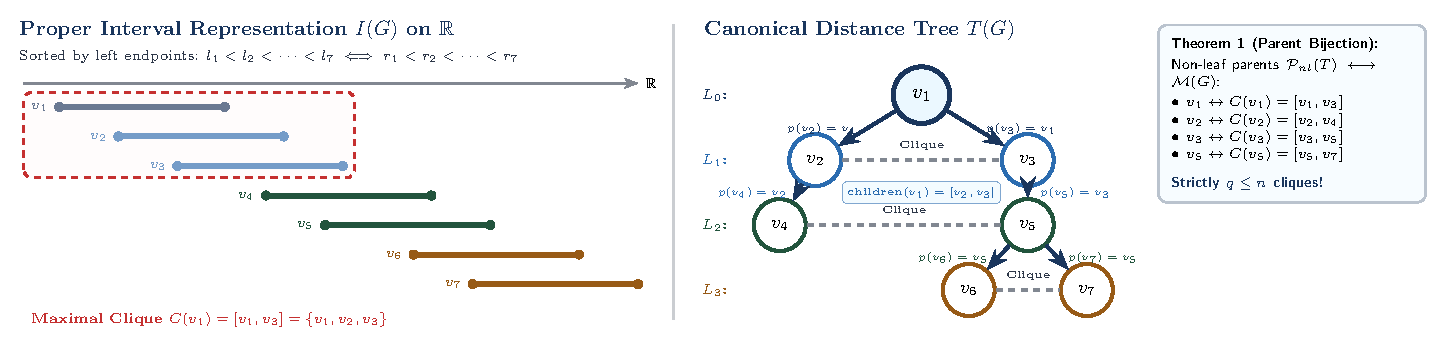
\includegraphics[width=0.95\linewidth]{figures/fig_distance_tree.pdf}
    \caption[Canonical Distance Tree $T(G)$ and Level Hierarchy]{Canonical Distance Tree $T(G)$ constructed on a proper interval graph. Depth levels $L_0, L_1, L_2$ decompose the vertex set according to shortest-path distance from root $v_1$. Canonical parent pointers $p(v)$ select the earliest reaching neighbor in the preceding level.}
    \label{fig:distance_tree}
\end{figure}

\subsection{Level Sets and Depth Decomposition}

The tree $T(G)$ partitions the vertex set $V$ into disjoint \emph{level sets} (or \emph{layers}) according to their tree depth, which corresponds exactly to their shortest-path distance from the root $v_1$:
\begin{definition}[Level Sets]
For each integer $k \ge 0$, the $k$-th depth level $L_k$ of $T(G)$ is:
\begin{equation}
    L_k = \{ v \in V \mid d_T(v_1, v) = k \} = \{ v \in V \mid d_G(v_1, v) = k \}.
\end{equation}
The \emph{height} of $T(G)$ is $h = \max_{v \in V} d_T(v_1, v)$. The levels form a partition of $V$:
\begin{equation}
    V = L_0 \cup L_1 \cup \dots \cup L_h, \quad \text{where } L_0 = \{v_1\} \text{ and } L_i \cap L_j = \emptyset \text{ for } i \ne j.
\end{equation}
\end{definition}

Within each level $L_k$, vertices inherit the canonical linear ordering:
\begin{equation}
    L_k = \langle u_{k,1}, u_{k,2}, \dots, u_{k,|L_k|} \rangle \quad \text{with} \quad l_{u_{k,1}} < l_{u_{k,2}} < \dots < l_{u_{k,|L_k|}}.
\end{equation}

\subsection{Fundamental Invariants of $T(G)$}

We establish three foundational structural properties of the canonical distance tree:

\begin{lemma}[Distance Encoding Property]
\label{lem:distance_encoding}
Let $G$ be a connected proper interval graph and $T(G)$ its canonical distance tree. For any vertex $v \in L_k$, the unique path in $T(G)$ from $v_1$ to $v$:
\begin{equation}
    \langle v_1 = p^k(v), \; p^{k-1}(v), \; \dots, \; p(v), \; v \rangle
\end{equation}
is a shortest path of length $k$ between $v_1$ and $v$ in $G$. Consequently, $d_G(v_1, v) = k$.
\end{lemma}
\begin{proof}
Because $T(G)$ is generated via Breadth-First Search, every edge $(p(v), v) \in E_T$ connects a vertex in $L_{i-1}$ to a vertex in $L_i$. By induction on $k$, the path in $T(G)$ has length exactly $k$. Since BFS discovers shortest paths in unweighted graphs, $d_G(v_1, v) = k$.
\end{proof}

\begin{lemma}[Level Adjacency Restriction]
\label{lem:level_adjacency_restriction}
Let $G$ be a connected proper interval graph and $T(G)$ its canonical distance tree. If $uv \in E$, then:
\begin{equation}
    |d_G(v_1, u) - d_G(v_1, v)| \le 1.
\end{equation}
That is, edges in $G$ exist only between vertices in the same level $L_k$, or between adjacent levels $L_k$ and $L_{k+1}$. No edge in $G$ can span across two or more levels ($uv \notin E$ if $|d_G(v_1, u) - d_G(v_1, v)| \ge 2$).
\end{lemma}
\begin{proof}
By the triangle inequality on shortest-path distances:
\[
    d_G(v_1, v) \le d_G(v_1, u) + d_G(u, v) = d_G(v_1, u) + 1.
\]
Symmetrically, $d_G(v_1, u) \le d_G(v_1, v) + 1$. Thus, $|d_G(v_1, u) - d_G(v_1, v)| \le 1$.
\end{proof}

\begin{lemma}[Parent Monotonicity]
\label{lem:parent_monotonicity}
Let $G$ be a proper interval graph ordered canonically. For any two vertices $u, v \in V$:
\begin{equation}
    u \le v \implies p(u) \le p(v).
\end{equation}
Furthermore, the set of children of any parent $p \in T(G)$, denoted $\operatorname{children}(p)$, forms a contiguous subsegment of the canonical ordering:
\begin{equation}
    \operatorname{children}(p) = [c_1(p), c_k(p)] = \{ w \in V \mid c_1(p) \le w \le c_k(p) \}.
\end{equation}
\end{lemma}
\begin{proof}
Suppose $u < v$. By definition, $p(u) = \arg\min_{x < u} \{l_x \mid r_x \ge l_u\}$. Since $u < v$, we have $l_u < l_v$, which implies $\{x \mid r_x \ge l_v\} \subseteq \{x \mid r_x \ge l_u\}$. Thus, any neighbor reaching $v$ from the left also reaches $u$. Because $p(v)$ is the minimum reaching neighbor for $v$, it must satisfy $p(u) \le p(v)$. 

Since the parent mapping $v \mapsto p(v)$ is weakly monotonic, the preimage $p^{-1}(p) = \operatorname{children}(p)$ is the inverse image of a single value under a monotonic function, which is necessarily a contiguous interval of indices $[c_1(p), c_k(p)]$.
\end{proof}

These preliminary properties establish that $T(G)$ imposes a deterministic, contiguous structural hierarchy on $G$. In Chapter~\ref{chap:structure}, we leverage this hierarchy to derive the complete parent-child and sibling clique theorems.
